\documentclass[10pt,twocolumn,letterpaper]{article}

\usepackage{cvpr}
\usepackage{times}
\usepackage{epsfig}
\usepackage{graphicx}
\usepackage{amsmath}
\usepackage{amssymb}
\usepackage{subcaption}

% Include other packages here, before hyperref.

% If you comment hyperref and then uncomment it, you should delete
% egpaper.aux before re-running latex.  (Or just hit 'q' on the first latex
% run, let it finish, and you should be clear).
\usepackage[breaklinks=true,bookmarks=false]{hyperref}

\cvprfinalcopy

\def\cvprPaperID{****} % *** Enter the CVPR Paper ID here
\def\httilde{\mbox{\tt\raisebox{-.5ex}{\symbol{126}}}}

% Pages are numbered in submission mode, and unnumbered in camera-ready
%\ifcvprfinal\pagestyle{empty}\fi
\setcounter{page}{1}
\begin{document}

%%%%%%%%% TITLE
\title{
    Better Image Super-Resolution Using Pixel-Wise Semantic Segmentations \\
    \large CS 381V Visual Recognition Final Project}

\author{Keivaun Waugh\\
University of Texas at Austin\\
{\tt\small keivaunwaugh@gmail.com}
% For a paper whose authors are all at the same institution,
% omit the following lines up until the closing ``}''.
% Additional authors and addresses can be added with ``\and'',
% just like the second author.
% To save space, use either the email address or home page, not both
\and
Paul Choi\\
University of Texas at Austin\\
{\tt\small choipaul96@gmail.com}
}

\maketitle
%\thispagestyle{empty}

%%%%%%%%% ABSTRACT
\begin{abstract}
In this paper, we address the problem of image super-resolution (SR) using
a ResNet based convolutional neural network (CNN) as well as a generative
adversarial network (GAN). Our approach differs from prior work with the
addition of explicit semantic segmentation data. We experiment with both
human annotated pixel-wise segmentations as well as machine generated
pixel-wise segmentations. Our results show that adding the segmentation
data to the network increases both quantitative and qualitative performance
of the SR network.
\end{abstract}

%%%%%%%%% BODY TEXT
\section{Introduction}
Image super-resolution is a compelling area of computer vision. Being able to
convert low resolution photos and video to higher resolution counterparts is an
important problem as hardware continues to improve. With higher resolution
displays and cameras more available today than ever before, it would be nice if
we could convert old media to the same resolution standards as current photos
and video. While image downsizing is an easy problem with a transformation that
can be easily specified, SR is an inherently underspecified problem. The goal
is to create an inverse transformation that ``hallucinates'' information from
the low resolution (LR) image to fill in the gaps for the high resolution (HR)
image. Naive methods of upsampling using nearest neighbor and bicubic
interpolation introduce many artifacts and produce visually displeasing images.
Figure 1 displays an example of results obtained with a naive method as well as
perfect results to which we aim to come closer.

\begin{figure}[ht]
    \begin{tabular}{cc}
            NN & Original \\
    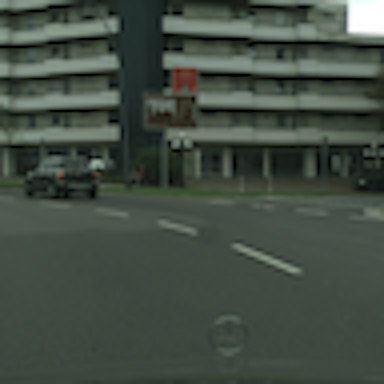
\includegraphics[trim=0 0 0 0, clip,
        width=1.5in]{images/example_lr_image.png} &
    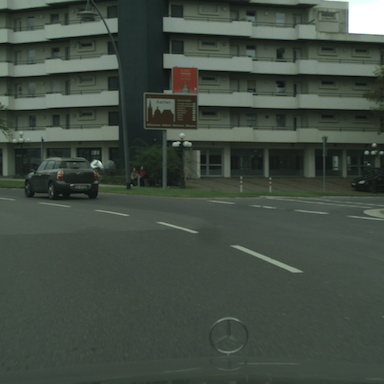
\includegraphics[trim=0 0 0 0, clip,
        width=1.5in]{images/example_hr_image.png} \\

    \end{tabular}
    \caption{Left: image upscaling using nearest neighbor. Right: The
    original image before downscaling then upscaling.}
    \label{fig:exampleIntroFirst}
\end{figure}

Deep networks have greatly increased in popularity for instance and category
recognition, sparked by work from Krizhevsky et al. \cite{AlexNet}. SR methods
based on deep networks have also achieved considerable success in SR tasks. We
use the success of these deep networks as a starting point for our research. In
this paper, we combine semantic segmentation features with state-of-the-art SR
techniques in order to achieve sharper SR solutions. We explain the intuition
behind adding this pixel-wise segmentation data later in this paper.

%------------------------------------------------------------------------------

\subsection{Related Work}
Before the advent of deep neural networks, basic approaches to SR were
available. The most naive is nearest neighbor which increases the resolution
with a simple pixel copy of the nearest pixel in between the LR and HR images.
A more common approach that typically gets better results and is the standard
in many image editors is bicubic interpolation.  However, neither of these two
methods attempt to use any kind of local or global structure in the image to
perform a better reconstruction.

Other, more advanced non-deep approaches exist for SR. Chung et al.
\cite{FractalSR} investigate the use of fractal patterns for the task of super
resolution. They were able to achieve better results than the naive methods.
Approaches for SR that involve video like those mentioned in Borman and
Stevenson's review \cite{VideoSR}. These algorithms aim to use context of
neighboring frames to pick values for the upsampled pixels. However, we choose
to stick to the problem of single image SR.

Dong et al. \cite{SRCNN} were the first to propose a CNN for the purpose of SR.
They used a basic deep architecture and trained their model end-to-end using a
per-pixel loss between the output and ground truth images. Johnson et al.
\cite{PerceptualLosses} proposed the use of a perceptual loss function for SR
to make the images more appealing to eye. They get worse quantitative results
such as peak signal-to-noise-ratio (PSNR) and structural similarity (SSIM), but
better qualitative results. This helped to motivate future work to use
perceptual metrics such as mean opinion score (MOS). Other similar work
involving CNNs for SR include \cite{RealtimeCNN} and \cite{DeeplyRecursive}.

Another more recent approach is to use a generative adversarial network (GAN)
\cite{GAN}. As mentioned previously, the CNN approaches typically attempt to
minimize the per-pixel loss between the upsampled output image and the original
unmodified image. The error metric frequently used is peak signal-to-noise
ratio (PSNR). However, when this is applied directly on the pixel space, this
often encourages the network to make soft changes in the upsampled image rather
than generate the high-frequency changes often found in real images. GAN based
approaches like the work of Ledig et al. \cite{SRGAN} attempt to overcome this
by using an adversarial network. Though they get lower PSNR values, the images
often look more realistic, which suggests that some other metric should be
optimized to get better results.

In \cite{ImageSynthesis}, Chen and Koltun experiment with using semantic
segmentation from the Cityscapes dataset \cite{Cityscapes} to perform
photorealistic image synthesis. The authors are able to get quote compelling
results using only the semantic segmentations as input to their CNN. However,
to our knowledge, there have been no papers published that attempt to merge
together this explicit semantic data with a SR technique for better results.

\subsection{Contribution}
Semantic segmentation is a core focus of much computer vision work. In this
paper, we are the first to explore the how the explicit addition of pixel-wise
semantic segmentation masks affect an SR network's ability to produce quality
results. We experiment with a high upscaling factor ($4 \times$). Our
hypothesis was that the segmentations will clean up ambiguous edges, especially
at high upscalings when the borders are especially fuzzy. We also evaluate the
effect of these segmentations on both more traditional ConvNet architectures as
well as GANs that have become more recently popular for the image generation
domain.

We describe our network architecture and segmentation pipeline in section
\ref{sec:method}. A quantitative evaluation of results is included in section
\ref{sec:evaluation}. Section \ref{sec:conclusion} contains concluding remarks
and a direction for future work based on our segmentation approach.

%------------------------------------------------------------------------------

\section{Method}
\label{sec:method}

Our solution to this task involves using a standard convolutional neural
network based on the ResNet architecture \cite{ResNet} as well as a generative
adversarial network \cite{GAN}. Both of these use modified architectures that
were designed by the authors of \cite{SRGAN}. We modified the input layers of
the generator network to take in the extra information supplied by the
segmentation pipeline. The two variants of this pipeline will be discussed in
future sections. When running the network in the standard ResNet mode, only the
generator is trained. When running in GAN mode, the generator is first
pretrained for $n$ epochs, followed by $m$ epochs of joint training between the
generator and the discriminator. Typically $n < m$, but this is not a hard
requirement.

\subsection{Architecture}
\begin{figure*}[ht!]
\begin{center}
    \begin{tabular}{c}
	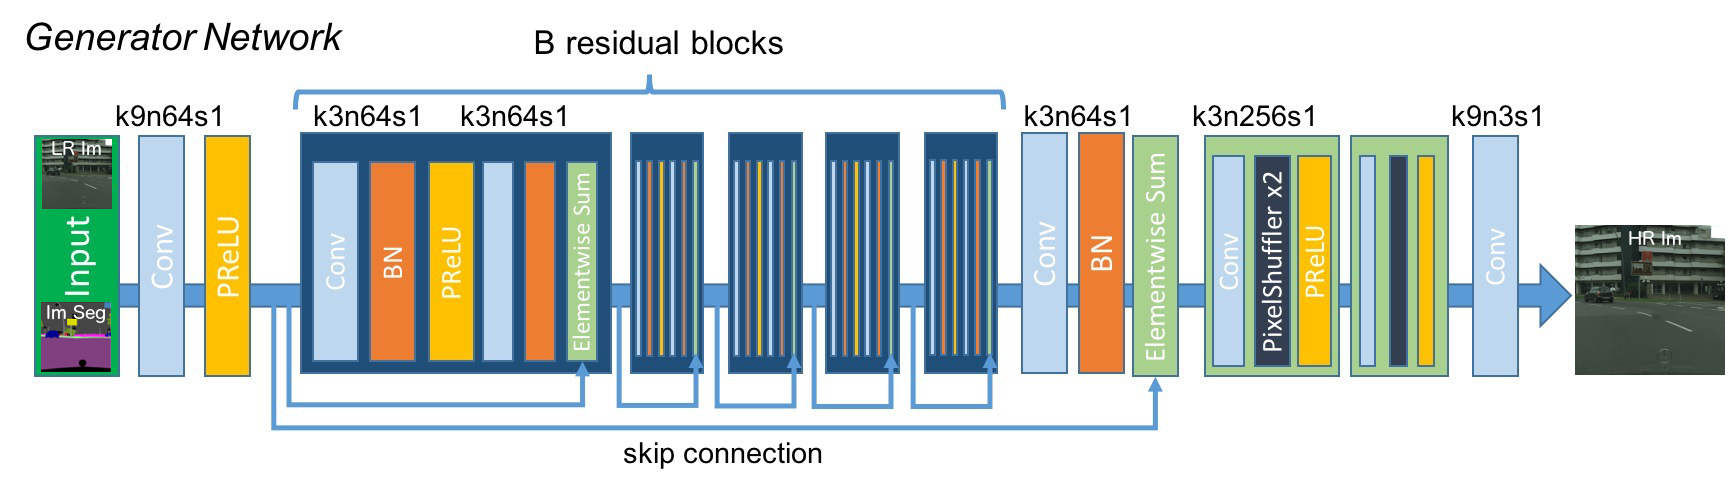
\includegraphics[width=6.5in]{images/generator_architecture.png}\\
	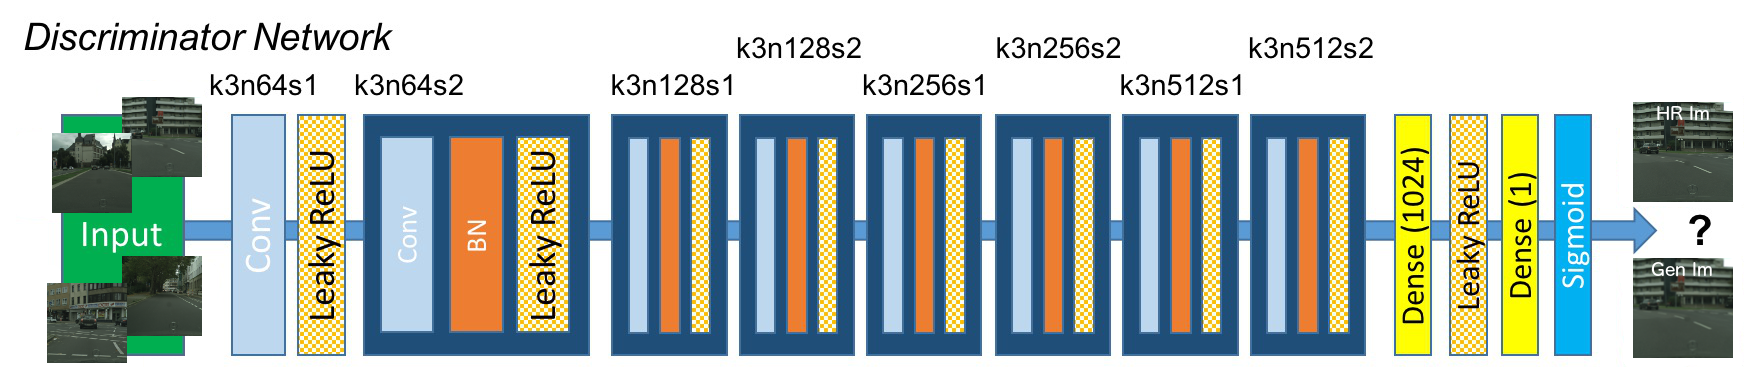
\includegraphics[width=6.5in]{images/discriminator_architecture.png}
    \end{tabular}
\end{center}
    \caption{Architecture of Generator and Discriminator Network with kernel
    size, feature map count, and stride at each layer in the network. Diagrams
    courtesy of \cite{SRGAN} as this was the basis of our architecture.}
    \label{fig:generator}
\end{figure*}

Figure \ref{fig:generator} illustrates the architectures for both the generator
and the discriminator.

\subsection{Human Segmentations}
All the datasets that we evaluated our system on contain human annotated
segmentations. These datasets are \cite{Cityscapes} and \cite{MSCOCO}. Due to
the large performance gap between current segmentation networks and human
annotated results, we wanted to evaluate our method in the best case possible
as a sanity test. If we were unable to get better results with the human
segemntations, then it would be unlikely that we were get better performance
with the machine segmentations at the present time, or even as they get better.
Not until they became significantly better than humans would there be a chance
of performance gains.

\subsection{Machine Segmentations}
Talk about reasons for using FCN \cite{FullyConvolutionalSS} over some other
solution that gets better performance. Discuss how it wasn't actually all that
crucial to get great performance out of the machine segmentations after we
showed that human segmentations get gains over no segmentations.

\begin{figure*}[ht!]
\begin{center}
    \begin{tabular}{ccc}
        Original & Human Segmentation & Machine Segmentation \\
    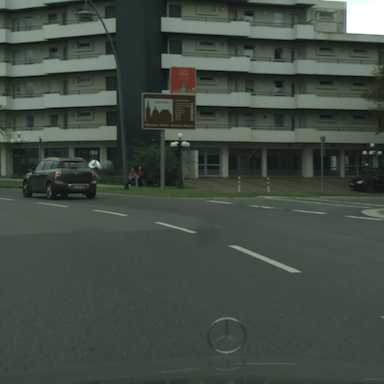
\includegraphics[trim=0 0 0 0, clip,
        width=2.0in]{images/segmentation_original.png} &
    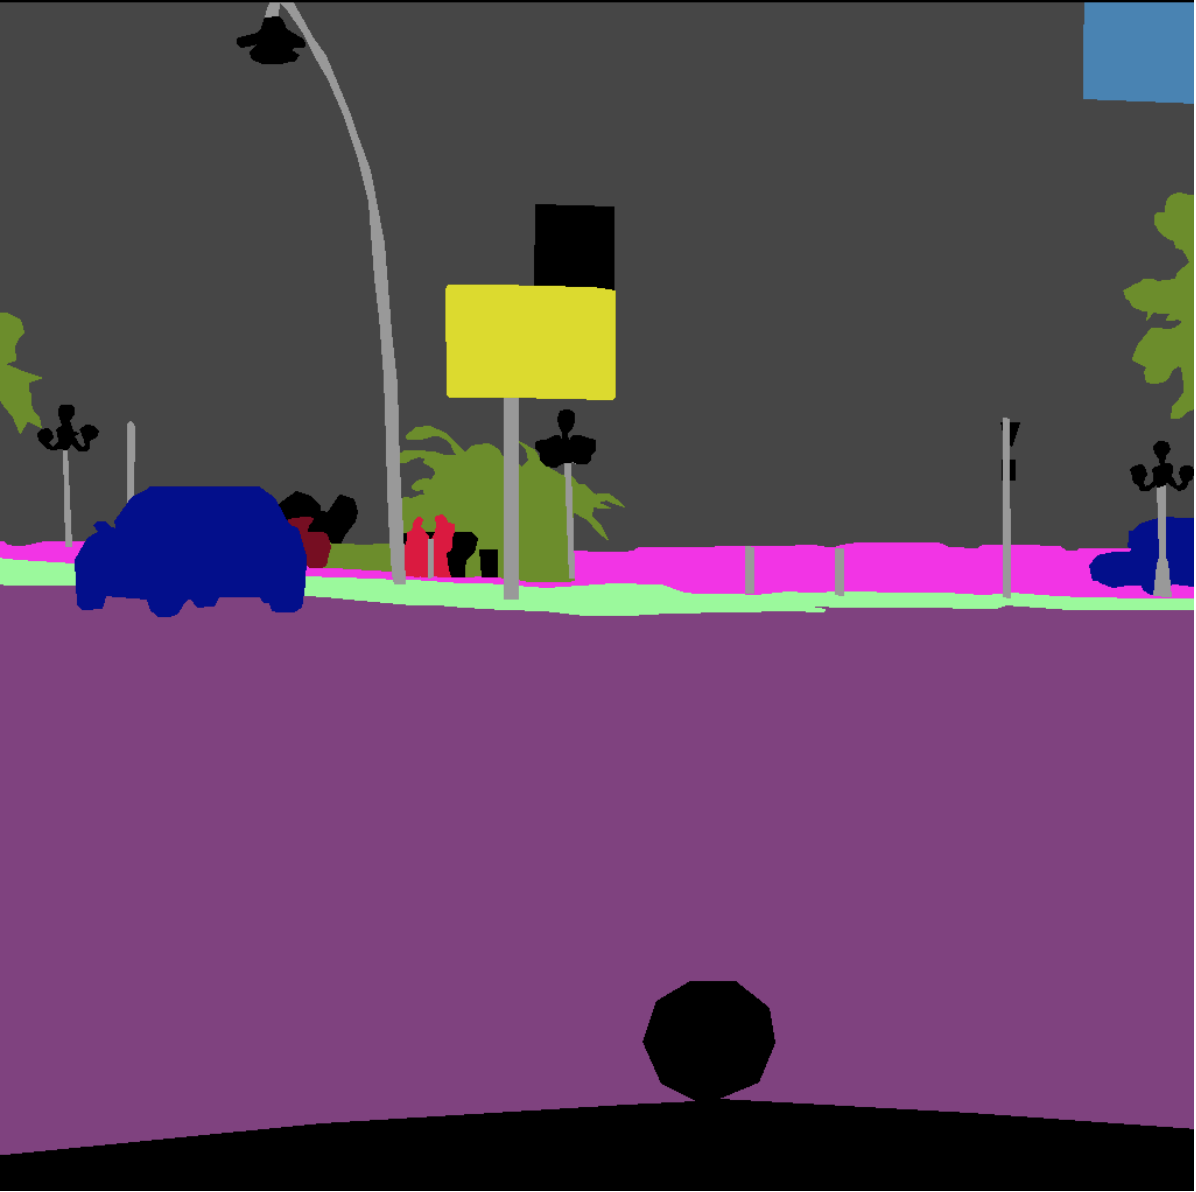
\includegraphics[trim=0 0 0 0, clip,
        width=2.0in]{images/segmentation_human.png} &
    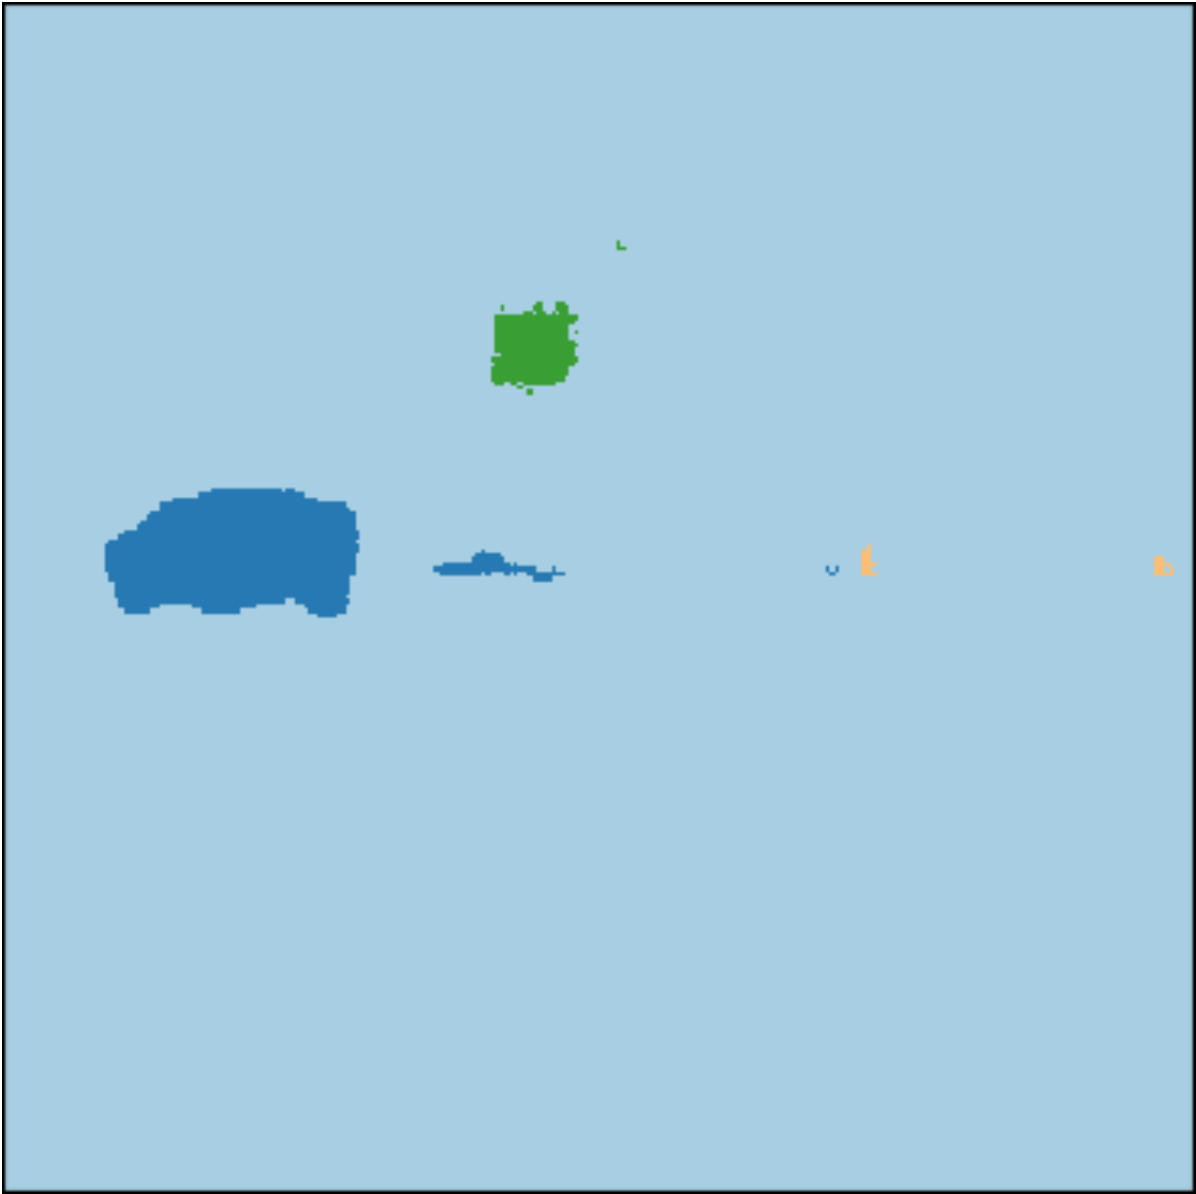
\includegraphics[trim=0 0 0 0, clip,
        width=2.0in]{images/segmentation_machine.png} \\
    \end{tabular}
\end{center}
                \caption{Comparison of segmentations between human generated
                and auto generated. Left: the original image. Middle: A human
                annotated pixel-wise semantic segmentation. Right: A machine
                generated segmentation.}
	\label{fig:segmentations}
\end{figure*}
%------------------------------------------------------------------------------

\section{Evaluation}
\label{sec:evaluation}
While discussing this problem with our peers, some have argued that if having
semantic segmentations added to the network would increase performance, the
vanilla GAN in \cite{SRGAN} should learn how to segment items in the scene
``under the hood''. We argued this was not true and pointed to \cite{ResNet} as
an example. The authors of this paper showed that it was difficult for deep
networks to learn identity mappings as the depth of networks increased. We
believed that a similar phenominon would occur in this domain and that adding
the segmentation information explicity, we could overcome this learning
difficulty. Our evaluations show that this is the case.

As is standard in other papers in this domain such as \cite{SRCNN},
\cite{SRGAN}, \cite{PerceptualLosses}, \cite{DeeplyRecursive}, we use the
metrics of peak signal-to-noise ratio (PSNR) and structural similarity (SSIM)
as quantitative measurements. However, as shown in \cite{SRGAN}, quantitative
measurements do not always translate to increases in perceptual qualtiy. As a
result, we have decided to adopt the use of a mean opinion score (MOS) and have
employed the use of our peers to help us gather data for this metric.

Filler

%------------------------------------------------------------------------------

\section{Technical Plan}
The authors of \cite{SRGAN} have their code for their SRGAN network available
online. We will use this code as a starting point and modify it to include our
semantic segmentation data from the datasets or out-of-the-box segmentation
networks. One method we will use for integration this additional data will be
to concatenate the segmentation data onto the feature maps of the early layers
in the network. This will be evaluated on both the traditional ResNet variant
that the authors introduce as well as the GAN version.

%------------------------------------------------------------------------------

\section{Experimental Plan}
We will build upon the open-source implementation of Ledig et al. \cite{SRGAN}
which uses TensorFlow 1.2. Our first task will be to apply the unmodified
network to a dataset of our choosing which includes semantic segmentation
labels. These results will constitute our baseline. We will use the same
measures to evaluate our SR method: PSNR, structural similarity (SSIM), and
mean opinion score (MOS). For MOS, we will conduct a survey as in \cite{SRGAN}
and ask raters to rate images produced by different methods on a scale of 1 to
5 in terms of quality. While the original paper uses 26 raters, we will likely
use fewer raters to ease the logistical burden. As an additional baseline, we
will also measure the performances of the nearest neighbor and bicubic
interpolation methods.

Our second and main task will be to modify the SRResNet and SRGAN networks to
utilize semantic segmentation features, as discussed in the technical plan. If
we have enough time, we will also experiment with adding these additional
features to the discriminator in the SRGAN network to see if it aids training.
The measurements from these modified approaches will indicate the effectiveness
of our method.

In addition to using a dataset with semantic segmentation labels, we will also
use datasets without such labels included and generate the labels manually
using an out-of-the-box solution. This will allow us to compare how
human-annotated segmentation features compare to machine-generated segmentation
features.

We will experiment with adding the segmentation data at multiple places in the
network. The most basic solution would be to add it onto the feature maps at
the earliest layers in the network. However, we plan to evaluate the network
with the segmentations included at different locations and multiple locations.

%------------------------------------------------------------------------------

\section{Sources of Data}
Image SR techniques are self-supervised in that explicit annotation of data is
unneeded. Given an image, a training pair can easily be generated by using the
downsampled image as the input to the SR network and the original image as the
ground truth. However, in order to integrate semantic segmentation knowledge,
we need to obtain the semantic layout for each image. There are two ways that we
plan on going about this. The first is to use datasets that already include
the segmentation such as the Cityscapes \cite{Cityscapes} dataset. The other
approach is to use existing segmentation networks as in
\cite{FullyConvolutionalSS} to generate the segmentation before the downsized
image is fed into our SR network. We plan to compare the results of the two to
see if the more accurate human-annotated segmentations are required to get good
results from our technique, or if a fully-automated SR approach can be achieved.

To compare our results against those obtained from other papers, we plan on
using standard evaluation datasets that are used in \cite{SRGAN}. These include
Set5 \cite{Set5}, Set14 \cite{Set14}, and BSD100 which is a subset of
BSD300 \cite{BSD300}

%------------------------------------------------------------------------------

\section{Partner Plan}
For the programming portion of the project, we plan to pair-program and
divide equally the implementation work. For experiments, we will individually
drive each one while working together as needed, with each person driving an
equal number of experiments. The report will be written collaboratively. The
person with more expertise on a given section will lead writing for that
section.

%------------------------------------------------------------------------------

\section{Speculation of Results}
Current state-of-the-art semantic segmentation methods already involve CNNs.
One may argue that a CNN based approach for SR would automatically learn
information regarding segmentation if it is useful for providing better
results. However, this argument does not take into account the difficulty of
learning such information. A parallel argument was made for residual networks
in \cite{ResNet} with regards to learning identity mappings. However, the
authors found that it was often difficult for networks to learn such mappings.
We predict that adding the semantic segmentation data explicitly to the network
will allow it to make more intelligent decisions along object boundaries. We
expect this will help provide crisper edges. Because of the success with using
semantic masks at various resolutions in \cite{ImageSynthesis}, we expect that
our results will be better at high upsampling factors.

\section{Experiments}
Filler

\section{Conclusion and Future Work}
\label{sec:conclusion}

\subsection{Omissions from Project Proposal}
I think in this section we should include a discussion of stuff that we said we
would do in the proposal that we didn't get around to doing in the final
project. We should justify why these were left out (whether it was because we
ran out of time, didn't think it would be that useful/sightful, etc.)

Filler

{\small
\bibliographystyle{ieee}
\bibliography{bib}
}

\end{document}
